%%% LaTeX Template: Two column article
%%%
%%% Source: http://www.howtotex.com/
%%% Feel free to distribute this template, but please keep to referal to http://www.howtotex.com/ here.
%%% Date: August 2017

%%% Preamble
\documentclass[	DIV=calc,%
							paper=a4,%
							fontsize=12pt,%
							onecolumn]{scrartcl}	 					% KOMA-article class

\usepackage{lipsum}													% Package to create dummy text
\usepackage[english]{babel}										% English language/hyphenation
\usepackage[protrusion=true,expansion=true]{microtype}				% Better typography
\usepackage{amsmath,amsfonts,amsthm}					% Math packages
\usepackage[pdftex]{graphicx}									% Enable pdflatex
\usepackage[svgnames]{xcolor}									% Enabling colors by their 'svgnames'
\usepackage[hang, small,labelfont=bf,up,textfont=it,up]{caption}	% Custom captions under/above floats
\usepackage{epstopdf}												% Converts .eps to .pdf
\usepackage{subfig}													% Subfigures
\usepackage{booktabs}												% Nicer tables
\usepackage{fix-cm}													% Custom fontsizes
\usepackage{float}
\usepackage[utf8]{inputenc}
\usepackage[top=2.5cm, bottom=2.5cm, left=2.5cm, right=2.5cm]{geometry}
\usepackage[ddmmyyyy]{datetime}
\addto\captionsenglish{%
	\renewcommand\tablename{Tabela}
	\renewcommand\figurename{Figura}
} 
 

 
%%% Custom sectioning (sectsty package)
\usepackage{sectsty}													% Custom sectioning (see below)
\allsectionsfont{%															% Change font of al section commands
	\usefont{OT1}{phv}{b}{n}%										% bch-b-n: CharterBT-Bold font
	}

\sectionfont{%																% Change font of \section command
	\usefont{OT1}{phv}{b}{n}%										% bch-b-n: CharterBT-Bold font
	}



%%% Headers and footers
\usepackage{fancyhdr}												% Needed to define custom headers/footers
	\pagestyle{fancy}														% Enabling the custom headers/footers
\usepackage{lastpage}	

% Header (empty)
\lhead{}
\chead{}
\rhead{}
% Footer (you may change this to your own needs)


\lfoot{\footnotesize \texttt{Cabeamento Estruturado} \textbullet ~Projeto São Borja}


\cfoot{}
\rfoot{\footnotesize página \thepage\ de \pageref{LastPage}}	% "Page 1 of 2"
\renewcommand{\headrulewidth}{0.0pt}
\renewcommand{\footrulewidth}{0.4pt}



%%% Creating an initial of the very first character of the content
\usepackage{lettrine}
\newcommand{\initial}[1]{%
     \lettrine[lines=3,lhang=0.3,nindent=0em]{
     				\color{DarkGoldenrod}
     				{\textsf{#1}}}{}}



%%% Title, author and date metadata
\usepackage{titling}															% For custom titles

\newcommand{\HorRule}{\color{DarkGoldenrod}%			% Creating a horizontal rule
									  	\rule{\linewidth}{1pt}%
										}

\pretitle{\vspace{-30pt} \begin{flushleft} \HorRule 
				\fontsize{50}{50} \usefont{OT1}{phv}{b}{n} \color{DarkRed} \selectfont 
				}


\title{Projeto de cabeamento estruturado Unidade}					% Title of your article goes here

%% ====================================



\posttitle{\par\end{flushleft}\vskip 0.5em}

\preauthor{\begin{flushleft}
					\large \lineskip 0.5em \usefont{OT1}{phv}{b}{sl} \color{DarkRed}}
\author{Diego Paulo Zoz }  	% Author name goes here


\postauthor{\footnotesize \usefont{OT1}{phv}{m}{sl} \color{Black} 
					\\Universidade Tecnológica Federal do Paraná - Campus Foz do Iguaçu 								% Institution of author
					\par\end{flushleft}\HorRule}

\date{}																				% No date




%%% Begin document
\begin{document}
\maketitle
\thispagestyle{fancy} 	
\thispagestyle{empty}		% Enabling the custom headers/footers for the first page 
% The first character should be within \initial{}


\initial{E}\textbf{ste projeto tem por objetivo reestruturar um estrutura real onde o cabeamento e toda a infraestrutura de rede é muito precária. Será necessário instalar Racks, patch panels, switches, novos pontos lógicos. A planta física e lógica será apresentada.}

%% ====================================
\begin{figure}
	\centering
	
\includegraphics{utfpr}
\end{figure}

\vspace{3cm}
\centerline{\textit{\textbf{\today}}}

%%\clearpage
  %%  \renewcommand*\listfigurename{Lista de figuras}
%%\listoffigures

%%\renewcommand*\listtablename{Lista de tabelas}
%%\listoftables

\clearpage
\renewcommand{\contentsname}{Sumário}
\tableofcontents
\clearpage

\section{Introdução}
Iremos reestruturar a rede da Unidade de negócio(Recebimento de grãos) localizada na cidade de São Borja-RS da empresa C.Vale. Este local foi recentemente adquirido e possui vários problemas na rede. O objetivo é regularizar tudo o que esta fora do padrão para solucionar problemas recorrentes que os colaboradores possuem e que prejudicam muito o desempenho do seu trabalho. O local possui aproximadamente 20 colaboradores, cada colaborador utiliza um computador para trabalhar e existem 3 impressoras que são ligadas na rede. 


\subsection{Benefícios}
\begin{itemize}
	
	\item A rede ficará estável, pois todo o cabeamento de rede será novo
	\item Serão instalados pontos de rede novos para todos os dispositivos, os pontos de redes atuais serão desativados após a conclusão do projeto
	\item Os pontos lógicos serão identificados, facilitando manutenções futuras ou mudança de ponto lógico para ponto de telefone no rack 
	\item Os outros prédios serão interligados com fibra óptica, aumentado a segurança e desempenho da rede
	\item Serão instalados Racks nos outros prédios, assim como pontos de rede.
\end{itemize}

\section{Estado atual}
A rede atual possui vários problemas:
o rack é pequeno e esta muito desorganizado, os patch cords não são certificados e possuem conectores com defeito, alguns pontos não estão crimpados no patch panel, não há identificação para os pontos lógicos, são utilizados pequenos switches em algumas estações de trabalho devido a falta de pontos de rede, a interligação do escritório com outros prédios(moegas, guarita, armazém) é feita via rádio ou com cabo UTP, não existe rack e pontos de rede estruturados nos outros prédios.

Segue alguns detalhes da rede atual:
\begin{itemize}
	\item 1 patch panel, cabo de rede, conectores, 1 Rack, etc
	\item a principal reclamação dos colaboradores são as paradas na rede, pontos de rede com mau contato, switches nas mesas desligam parando a rede de toda uma ilha de computadores, lentidão.
\end{itemize}


\section{Usuários e Aplicativos}
Atualmente todos os usuários utilizam computadores que estabelecem uma conexão RDP com um servidor da Sede da empresa. Todos os aplicativos necessários para o dia a dia de trabalho ficam nesse servidor, assim como o ERP. Impressoras são ligadas na rede e são instaladas nos servidores também. É provável que a quantidade de usuários aumente quando a empresa implantar o setor de acessório de peças na Unidade.
 

\subsection{Usuários}
Os usuários atuais são divididos da seguinte forma: 1 gerente, 1 subgerente, 2 balanceiros, 3 financeiro, 4 agrônomos, 4 vendedores de insumos, 1 caixa, 1 zeladora, 1 classificador, 2 insumistas.

\subsection{Aplicativos}
Os usuários utilizam basicamente o aplicativo de RDP em seus computadores. No caso do micro computador da balança, possui um software específico que faz a captura do peso da mesma.

\section{Estrutura predial existente}

A unidade é composta por 4 prédios: escritório, guarita, armazém e moegas.

A Figura \ref{fig1} representa a planta do escritório. 

\begin{figure}[H]
	\centering
	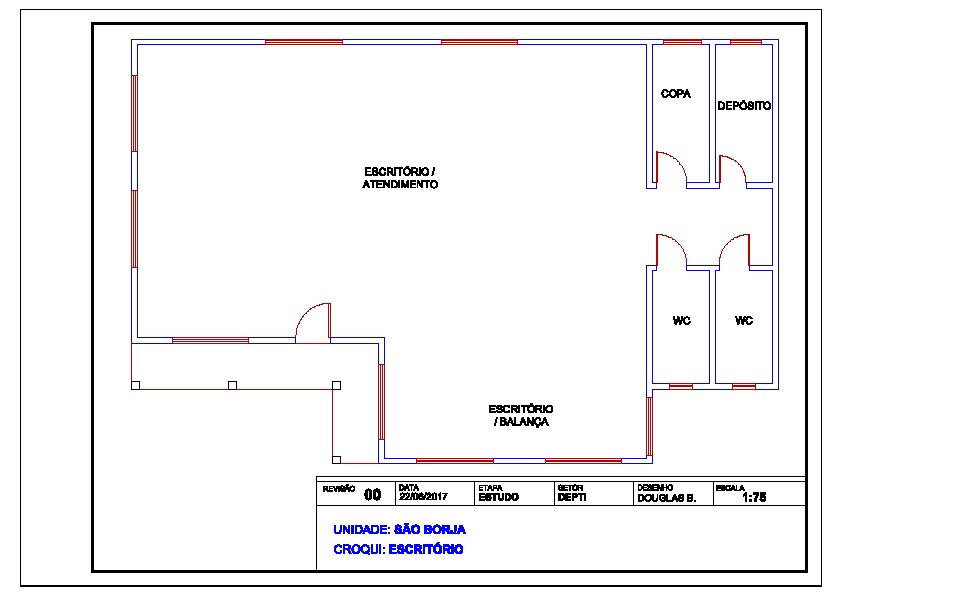
\includegraphics[width=\textwidth]{fig1}
	\caption{Layout Escritório}
	\label{fig1}
\end{figure}

A Figura \ref{fig2} representa o layout do patio da Unidade, com a previsão de interligação com dutos subterrâneos para passagem de fibra óptica.

\begin{figure}[H]
	\centering
	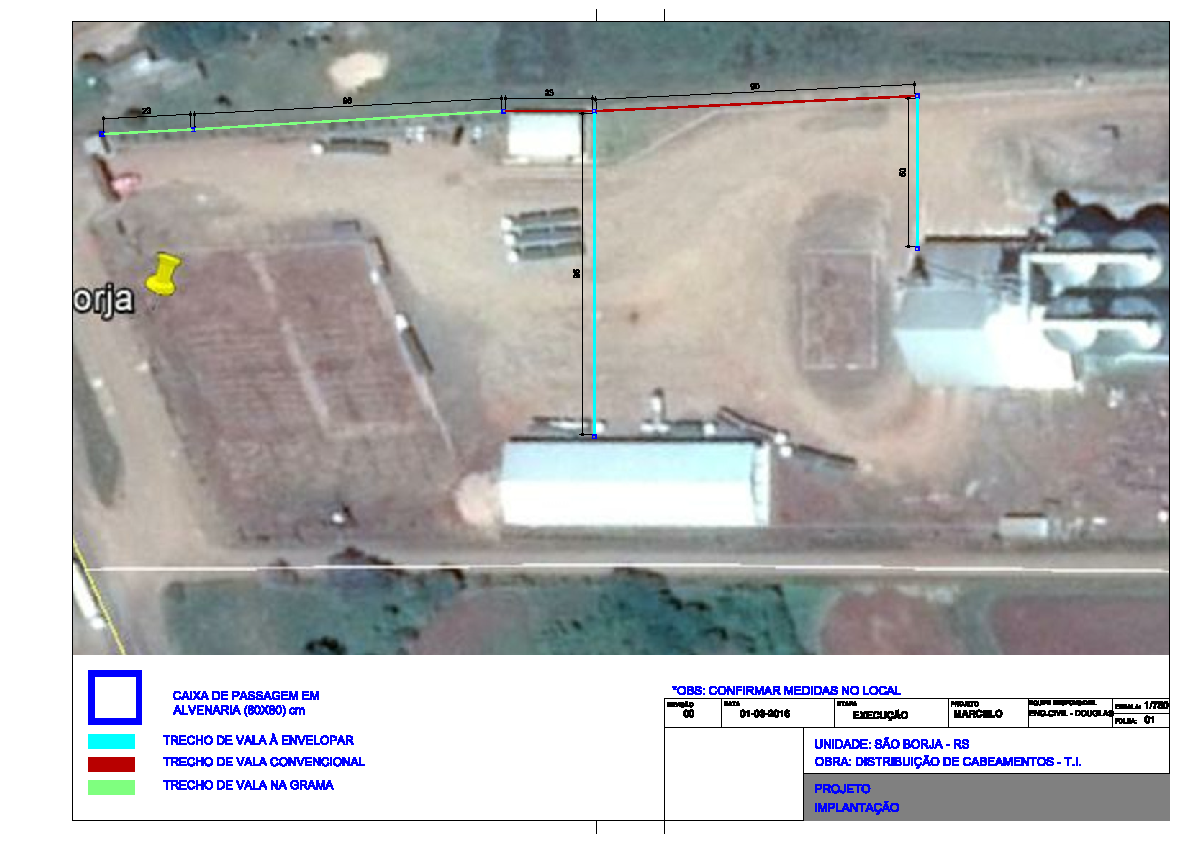
\includegraphics[width=\textwidth]{fig2}
	\caption{Layout Pátio}
	\label{fig2}
\end{figure}

\section{Planta Lógica - Elementos estruturados}

\subsection{Estado atual}
A planta atual não possui pontos de rede para atender todos os terminais da maneira com estão dispostos

\subsection{Topologia}

A Figura \ref{fig3} mostra a identificação dos pontos de rede e infra estrutura que será executada.

\begin{figure}[H]
	\centering
	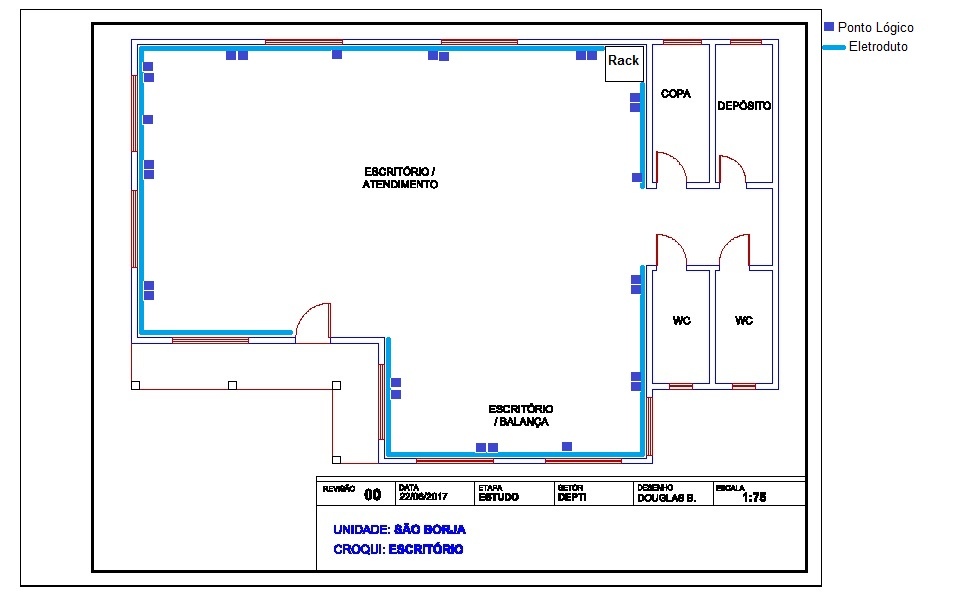
\includegraphics[width=\textwidth]{fig3}
	\caption{Pontos Lógicos}
	\label{fig3}
\end{figure}

A Figura 4 identifica como ficará o Rack do escritório após a implantação.

\begin{figure}[H]
	\centering
	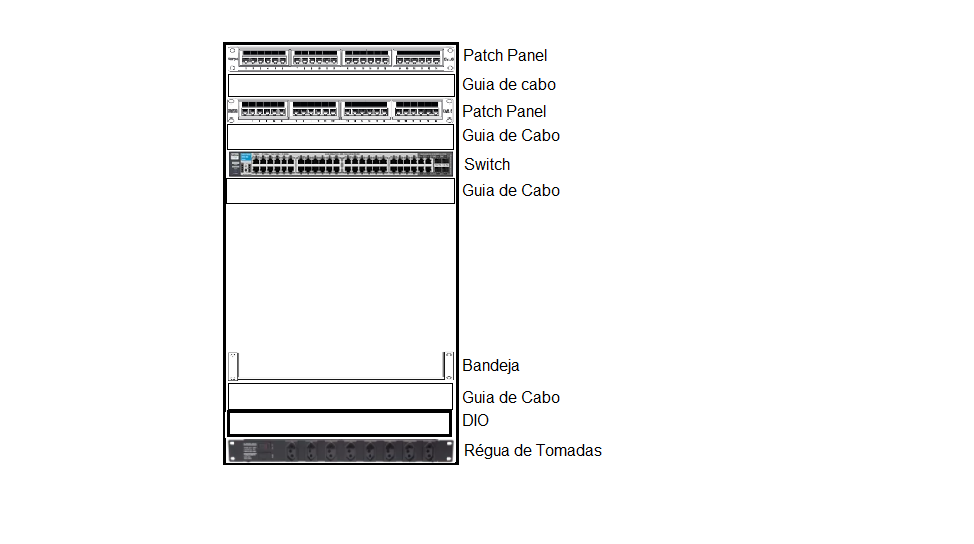
\includegraphics[width=\textwidth]{fig4}
	\caption{Rack Escritório}
	\label{fig4}
\end{figure}

A Figura 5 identifica como ficará o Rack dos prédios da guarita, armazém e moegas após a implantação.

\begin{figure}[H]
	\centering
	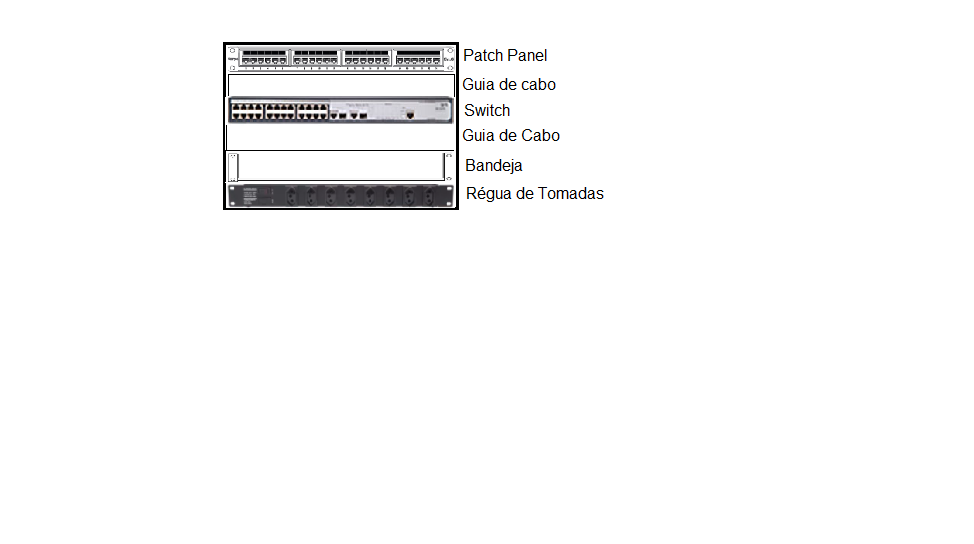
\includegraphics[width=\textwidth]{fig5}
	\caption{Racks Guarita, Armazém e Moega}
	\label{fig5}
\end{figure}

%%\begin{table}[h!]
\centering
\caption{Exemplo de tabela explicativa}
\label{tab1}
\begin{tabular}{|l|l|l|}
\hline
\multicolumn{3}{|l|}{Figura na Tabela} \\ \hline
1        & Rack          & 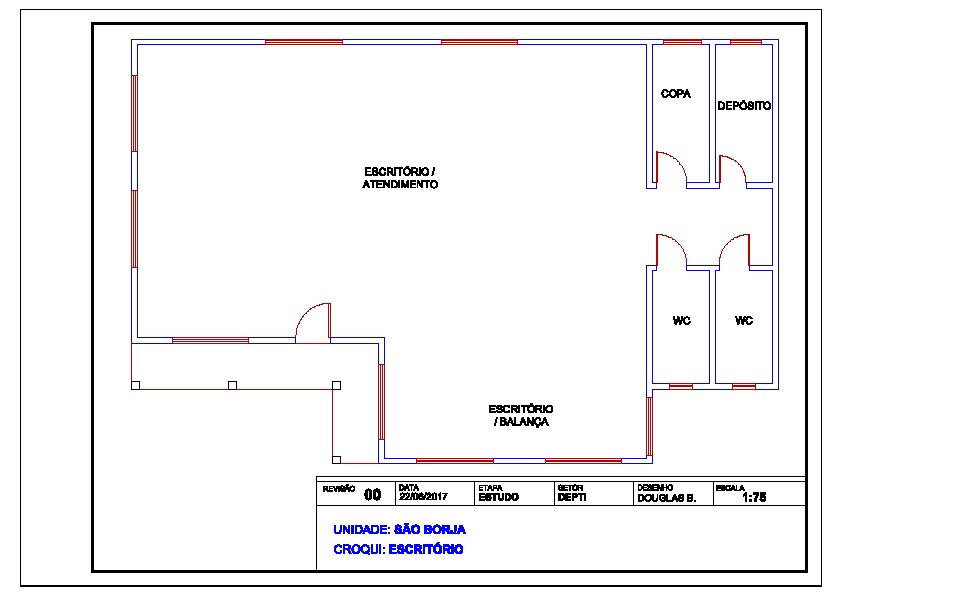
\includegraphics[scale=0.2]{fig1}        \\ \hline
2        & Rack 2        & 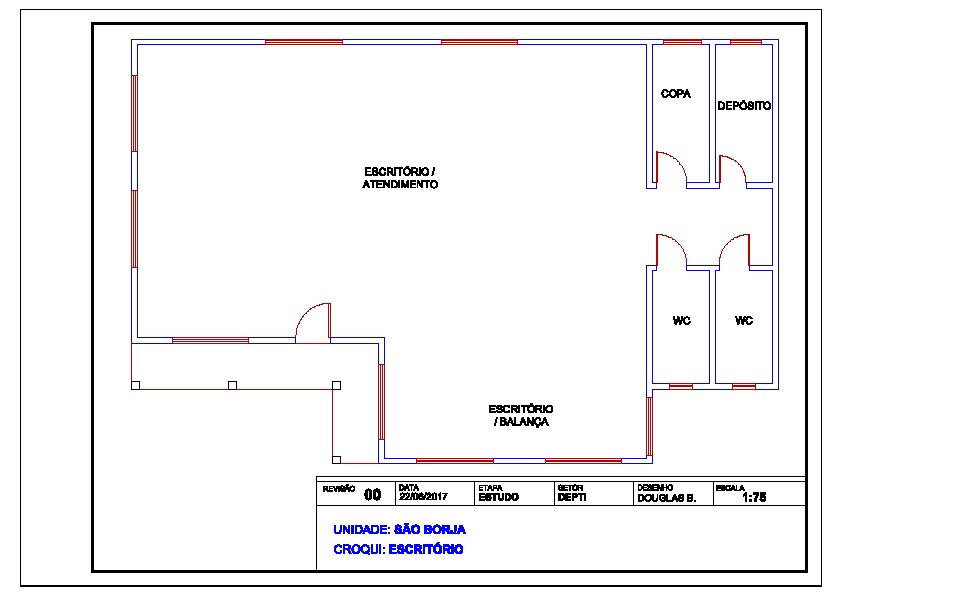
\includegraphics[scale=0.2]{fig1}        \\ \hline
\end{tabular}
\end{table}

\subsection{Encaminhamento}
Os cabos serão passados dentro de eletrodutos e perfilados. 

\subsection{Memorial descritivo}
Materiais que serão utilizados:
\begin{itemize}
	\item 5 patch panels Standard Furukawa
	\item 1 Rack 16U Attic
	\item 3 Racks 6U Attic
	\item 32 conectores RJ45 Fêmea Standard Furukawa
	\item 960m de cabo de rede CM Furukawa Cat.5e
	\item 10 guias de cabo
	\item 4 réguas de tomadas para rack
	\item 4 bandejas para rack
	\item 32 patch cords 1,5m Furukawa Cat.5e
	\item 32 patch cords 2,5m Furukawa Cat.5e
	\item 450m Fibra óptica AR 4FO Furukawa
	\item 12 extensões ópticas LC
	\item 1 DIO de rack
	\item 3 Mini DIO de Rack
\end{itemize}

\subsection{Identificação dos cabos}
Serão utilizado cabos Furukawa CM categoria 5e. Não ha necessidade de comunicação Gigabit localmente.

\section{Implantação}

Cronograma de implantação:
\begin{itemize}
	\item Instalação dos eletrodutos e conduletes
	\item Passagem dos cabos de rede pela infra estrutura
	\item Passagem da fibra óptica entre os prédios
	\item Instalação dos novos racks
	\item Crimpagem dos cabos no racks e nos pontos
	\item Identificação dos pontos lógicos e uplinks de fibra óptica
	\item Mudança dos equipamentos onde chega o link de internet da Unidade para o novo Rack do escritório e instalação dos patch cords nos novos pontos de rede, ligando nos dispositivos a fins. (Esta etapa será executada fora do horário de expediente, para não impactar no atendimento ao público na Unidade, pois haverá interrupção no acesso ao sistema)
	\item Remoção do rack atual
	\item Remoção dos rádios que fazem alguns uplinks nos prédios do local.
\end{itemize}
Todo o serviço será realizado por uma empresa terceira. Previsão de 12 dias para execução do projeto.


\subsection{Plano de expansão}
Todos os locais terão portas de rede sobrando nos switches e patch panel, onde houver, para necessidade de expansão futura. Caso haja necessidade, também haverá espaço nos racks para instalação de mais passivos e ativos.

\section{Orçamento}
Fornecedor 1: 15 mil reais de material e 10 mil reais de mão de obra.


Fornecedor 2: 15 mil reais de material e 9 mil reais de mão de obra.



\end{document}